\chapter{State of the Art}
\label{sota}
We examined a broad range of different topics with social media as central subject. It was an evolution starting from straightforward Twitter-related subjects to a full-fledged problem assignment many people struggle with.

This chapter is subdivided into two main parts. The first part (\autoref{technologies}) is a summary of the different technologies we examined in regard with the problem statements together with a short explanation. The second part (\autoref{opinionmining}, \autoref{twitterinfluencers} and \autoref{expertfinding}) gives a chronological overview of thesis topics we examined. For each topic there are several references to technologies described in the first part which could be useful in solving the problem.


\section{Technologies and Techniques}
\label{technologies}

%\subsection{What do we need}

%%%%%%%%%%%%%%%%%%%%%%%%%%%%%%%%%%%%%%%%%%%%%%%%%%%%%%%%%%

%% Several components we still have to explain or discuss inside the text %%

\subsection*{API}
\label{api}

API stands for Application Programming Interface and is a particular set of rules defined in code allowing software programs to communicate with each other. It facilitates the interaction by providing an interface for all the allowable actions.

We will use API's when they are available for obtaining information from online sources.

\subsection*{Web scraping}
\label{scraping}

Web scraping (also called Web harvesting or Web data extraction) is a computer software technique of extracting information from web sites. Usually, such software programs simulate human exploration of the Web by implementing low-level Hypertext Transfer Protocol (HTTP). Web scraping focuses on the transformation of unstructured data on the Web, typically in HTML format, into structured data that can be stored and analyzed in a central local database or spreadsheet. 

We will mainly use it to extract information of online sources if it lacks a decent API.

%% TODO : verzetten! Deze opsomming van sources zou beter vermeld worden bij plugins, deze zijn niet echt nodig in dit hoofdstuk

%\subsection{DBLP}
%
%DBLP is produced by the Computer Science department of the University of Trier and was initially focused on \textit{DataBase systems and Logic Programming}, but has gradually expanded toward being an confidential server providing bibliographic information on major computer science journals and proceedings, indexing more than one million articles.
%DBLP allows to search by author name, giving back a list of publications and other bibliographic information.
%
%DBLP does not provide us with an API, so we will use web scraping in order to extract all the necessairy information.
%
%%Link naar de volledige uitleg van de werking van de plugin voor meer informatie hieromtrent
%
%\subsection{LinkedIn}
%
%LinkedIn is a business-related social networking site launched in May 2003, mainly used for professional networking by more than 100 million registered users \footnote{http://en.wikipedia.org/wiki/LinkedIn}. Each user has a profile which may contain the following information: current affiliation and title, past working experiences, education, specialties, location, connections with other users...
%
%Using the LinkedIn API we can search for users by entering a name. This will give back list of profiles we can browse and whose information we can extract and use in our framework. As the service is based on a \textit{gated-access approach}, which means you need to be at least a second level connection of the profile you are looking at to see their connections, we can not use this to connect authors to eachother. However, the information provided by the profile which is publicly available does allow us to get a better insight into the subject the person is interested in and what affiliation he is and was connected to.
%
%%Link naar de volledige uitleg van de werking van de plugin voor meer informatie hieromtrent
%
%\subsection{Google Scholar}
%
%Google Scholar is a freely accessible web search engine that indexes the full text of scholarly literature accross an array of publishing formats and disciplines. It allows to search publications based on subject keywords, partial publication titles and author names. It's ranking algorithm uses a combination of factors, but puts mainly high weight to citation count and the words included in a document's title.
%
%Google Scholar is not yet available to the Google AJAX API and Google does not allow automatic crawling or scraping of its services. Thus, it can not be used as a publication reference in our framework.
%
%\subsection{Microsoft Academic Search}
%
%Microsoft Academic Search is a free search engine for academic papers and resources principally in the field of computer science, developed by Microsoft Research Asia, Beijing. The database consists of the bibliographic information (metadata) for academic papers published in journals, conferences proceedings and the citations between them. Objects are ranked according to two factors: their relevance to the query, which is computed by its attributes; and their global importance, calculated by its relationships with other objects \footnote{http://en.wikipedia.org/wiki/Microsoft Academic Search}.
%
%It is a direct competitor of Google Scholar and it allows us to scrape the information of the site, making it useful to extract publications written by a specific author, his fields of interest, the amount of times he was cited and his co-authors for our framework.

\subsection*{OWL}
\label{owl}

The Web Ontology Language or OWL is a family of knowledge representation languages for authoring ontologies, which represents a set of concepts within a domain and the relationships between these concepts. OWL is designed for applications that need to process the content of information instead of just representing it.

\subsection*{FOAF}
\label{foaf}

FOAF, or Friend of a Friend, is a descriptive vocabulary expressed using the Resource Description Framework (RDF) and the Web Ontology Language (OWL). It is an ontology used for describing persons, their activities and relationships to other people and objects. Each profile has a unique identifier, used for defining these relationships.

\subsection*{Freebase}
\label{freebase}

Freebase is a publicly available, collaborative entity graph describing people, places and objects and relationships between these entities. It is an online collection of structured, cross-linked data providing an interface to access common information more effectively. One way this could be used is to find relationships between words. As synonyms and alternative spelling are also included, it allows to determine a central subject in messages where the same word is written differently.

\subsection*{Stemming}
\label{stemming}

In linguistic morphology, stemming is the process for reducing inflected (or sometimes derived) words to their stem, base or root form � generally a written word form. The stem need not be identical to the morphological root of the word; it is usually sufficient that related words map to the same stem, even if this stem is not in itself a valid root. 

Algorithms for stemming have been studied in computer science since 1968. The Porter stemming algorithm \cite{porter1980algorithm} dates back to 1980, but is very widely used and the de-facto standard for the English language.

Closely related to stemming is lemmatisation, the algorithmic process of determining the lemma for a given word. The difference is that a stemmer operates on a single word, while a lemmatiser also has knowledge of the context. Stemmers typically run faster and the reduced accuracy may not matter for some applications.

\subsection*{Clustering}
\label{clustering}

Cluster analysis or clustering is the assignment of a set of observations into subsets (called clusters) so that observations in the same cluster are similar in some sense. Clustering is a method of unsupervised learning and is a common technique for statistical data analysis.

There are a lot of different graph clustering algorithms. Algorithms based on spectral clustering \cite{kannan2000clusterings}, multilevel graph partitioning schemes like METIS \cite{karypis1999fast} and the MLKM algorithm \cite{dhillon2005fast}. 

More recently there has been a new direction to graph clustering, modeling the minimum-cut, maximum-flow problem of the underlying graph \cite{flake2004graph}. The algorithm we will use is the dynamic version described in \cite{saha2006dynamic}. It is a dynamic algorithm based on the minimum-cut tree problem. It produces a high quality of clusters without having to look at the entire graph but only a subset of nodes, severely reducing the time of the algorithm.


\subsection*{Machine learning}
\label{machinelearning}

Machine learning, part of artificial intelligence, focuses on the development of algorithm that allow computer programs to learn from experience (ie. predicting the next event given a list of previous ones). This can be obtained by constructing rules and constraints, starting from some training data.

There are many different approaches with different computational performances. With regard to Opinion Mining, described in \autoref{opinionmining}, the most interesting is probably support vector machines which uses a set of related supervised learning methods for classification and regression. Clustering is also a form of machine learning and has already been explained in more detail in \autoref{clustering}.

\subsection*{Fuzzy String matching}
\label{stringmatching}

Fuzzy string matching is the technique of finding strings that match a pattern approximately (rather than exactly). Very different methods of string matching exist. Most of them either use a distance metric or a similarity metric. An example of an algorithm measuring the distance between two string is the Jaro-Winkler algorithm. The Jaro�Winkler distance metric is designed and best suited for short strings such as person names. A comparison of this algorithms with others can be found in \cite{cohen2003comparison}.

An example of an method using a similarity metric is Dynamic Time Warping. In general, DTW is a method that allows a computer to find an optimal match between two given sequences (e.g. time series) with certain restrictions. The sequences are "warped" non-linearly in the time dimension to determine a measure of their similarity independent of certain non-linear variations in the time dimension.

\subsection*{Part-Of-Speech Tagger}
\label{postagger}

%http://nlp.stanford.edu/software/tagger.shtml

A Part-Of-Speech Tagger, or POS Tagger, is a piece of software that reads text in some language and assigns parts of speech to each word. With parts of speech we mean nouns, verbs, adjectives, etc. Generally computational applications will use more fine-grained POS tags like 'noun-plural'. 

The POS Tagger we refer to is the Stanford Part-Of-Speech Tagger. This is a Java implementation of the log-linear part-of-speech taggers described in the papers \cite{toutanova2000enriching} and \cite{toutanova2003feature}. The software can be downloaded from \cite{postagger}.

There is also a Ruby port of the Lingua::EN::Tagger, called EngTagger, available as a gem. Documentation can be found at \cite{engtagger}.

\subsection*{Graph pattern-matching and Gremlin}
\label{graphs}

Gremlin is a domain specific language for traversing property graphs. Gremlin makes use of Groovy and Pipes to perform complex graph traversals. This language has application in the areas of graph query, analysis, and manipulation. One of the techniques used in Gremlin is graph pattern matching. Many graph applications have to do with identifying patterns in the graph. That is, identifying sub-graphs that match a particular topology and/or feature set. In single-relational graphs, usually a topology is only considered. An interesting article about pattern matching can be found at \cite{markopatterns}.

\subsection{JUNG}

JUNG (the Java Universal Network/Graph Framework) is a software library that provides a common and extensible language for the modeling, analysis, and visualization of data that can be represented as a graph or network. It is written in Java, which allows JUNG-based applications to make use of the extensive built-in capabilities of the Java API, as well as those of other existing third-party Java libraries.

The JUNG architecture is designed to support a variety of representations of entities and their relations, such as directed and undirected graphs, multi-modal graphs, graphs with parallel edges, and hypergraphs. It provides a mechanism for annotating graphs, entities, and relations with metadata. This facilitates the creation of analytic tools for complex data sets that can examine the relations between entities as well as the metadata attached to each entity and relation.

JUNG comes with implementations of well known graph-algorithms and visualization algorithms which might be very useful.

\section{Opinion mining}
\label{opinionmining}

\label{general - opinion mining}
Opinion mining is part of the general area of \textit{sentiment analysis, opinion extraction or opinion mining and feature-based opinion summarization} from the user-generated content or user-generated media on the Web. The applications are manifold with the most important ones in the area of in business intelligence. 

An example is a large company who wants to follow up on customer feedback. Large companies receive thousands of pieces of feedback on a daily basis, both direct as indirect. This feedback can exist out of online customer reviews, customer feedback, survey responses, social media messages or blogposts. Human processing of such text volumes is prohibitively expensive and close to impossible. The only alternative is automatic extraction of relevant information. Ideally one would like to be able to quickly and cheaply customize a system to provide an overview of the most interesting pieces of feedback which should be responded to or an overview of the general sentiment classification.

\subsection{Current situation}

%Sentiment360, lots of papers and onderzoek, really to much to name and to add something of importance.

Opinion mining has been a hot topic the last 10 years due to the rise of social media such as blogs and social networks. Businesses have a need to know what people are saying about them and opinion mining can help them toward accomplishing this goal \cite{wright2009mining}.

Several universities around the world have research teams focusing on the dynamics of sentiment. There is research focused on creating sentiment summaries to capture an author's opinion about a subject based on a publication \cite{beineke2003exploration}, predicting the semantic orientation of adjectectives and combinations of adjectives \cite{hatzivassiloglou1997predicting}, identifying the sources of the opinions rather than the actual sentiment itself \cite{choi2005identifying} and so on.

An interesting ongoing project is \cite{liu2004sentiment} at the University of Illinois, Chicago, backed by Google and Microsoft Corporation. It is a project focusing on three areas: 

\begin{itemize}
	\item Mining direct (or regular) opinions. Example: after taking the drug, I got stomach pain.
	\item Mining comparative opinions. Example: Coke tastes better than Pepsi.
	\item Review and opinion spam analysis and detection. An example is detecting of fake reviews.
\end{itemize}

It is particularly interesting as others can follow the status of and updates on the project. There are also references to the opinion lexicon and data sets they used to evaluate their results allowing third parties to compare their own work using the same input.

% TODO include a table comparing some existing pieces of software, comparing the pro's and con's ?

\subsection{Improvements and additions}

It could be interesting to work out previous research experiments with a focus on Twitter. The short and typically cryptic messages exchanged by users on this service form a new challenge where existing solutions may fall short as users often use shorthand codes, acronyms and abbreviations which are not part of the official language. A new approach or combination of existing solutions could be tested and compared to existing results.

There are many possible approaches. We could focus on the use of a log-linear regression model to predict the semantic orientation of adjectives and conjunctions \cite{hatzivassiloglou1997predicting}. Another possibility is a holistic lexicon-based approach which exploits external evidences and linguistic conventions of natural language expressions allowing to handle opinion words that are context dependent \cite{ding2008holistic}. In \cite{mei2007topic} a specifically designed Hidden Markov Model structure is utilized to track opinions in weblogs. In \cite{beineke2003exploration} a Naive Bayes and regularized logistic regression models are composed in order to capture opinions from online reviews.

Most of the approaches use some sort of classification algorithm or machine learning technique (\autoref{machinelearning}) in order to correctly predict opinions in a new context. In order to only consider interesting words, we would use a part-of-speech tagger (see \autoref{postagger}). This allows us to strip all the words that do not influence an opinion. On the remaining words, we would use a Stemming algorithm or a Lemmatizer (\autoref{stemming}).

% TODO waarom hebben we dit niet gekozen ? 


\section{Twitter influencers}
\label{twitterinfluencers}

As discussed in \autoref{general - opinion mining} about opinion mining, people talk about products, both positive as negative. They have the ability to influence the buying behavior of others who respect their opinion about a certain area. Identifying these influencers can be of great value, for instance in the advertising industry.

There are two main aspects, reach and trust. A person's reach determines the number of people who listen when he has something of value to say. Trust depicts the value people give a certain person's opinion. Both aspects can vary a lot when comparing different topics for the same person.

\subsection{Current situation}

There are papers discussing algorithms to find the ideal subset of individuals which will trigger a large cascade of conversions \cite{kempemax} and papers researching the more general economic issues regarding influencers \cite{kleinberg2007cascading}.

Also regarding the second aspect, trust, there are a lot of well documented scientific results. \cite{ziegler2005propagation} describes propagation models which can be used to present trust and distrust in social networks. Just as in \cite{golbeck2006inferring} an algorithm for calculating a trust metric is presented based on the EigenTrust algorithm\cite{kamvar2003eigentrust}.

The amount of applications focusing on calculating social media influence, as their core business or a useful option, is growing rapidly. An overview of a very limited set of interesting applications and what makes them special can be found in \autoref{tab:influenceApps}.

% TODO nog andere applications ? Andere soort mss ?
 
\begin{table}
	\centering
		\begin{tabular}[ht] {| m{3.5cm} | p{10cm}|}
			\hline
			
\includegraphics[width=3cm]{./fig/klout-logo-1.png} \cite{klout}	& Probably the best-known online tool focusing on ranking Twitter profiles (and recently also Facebook profiles) using over 35 variables. These rankings are, though fun, not particularly useful as finding influencers based on topic is very limited. However there are interesting third-party applications providing this feature.\\ 
			\hline
			
\includegraphics[width=3cm]{./fig/peerindex_logo.png} \cite{peerindex} & This application focuses on identifying topics which Twitter users talk about. Starting in 2011 they also have a commercial program which allows users to identify 'opinion formers and authorities', which comes down to identifying Twitter influencers.\\
			\hline
			
\includegraphics[width=3cm]{./fig/traackr_logo.png} \cite{traackr} & Traackr does not limit itself to Twitter. It uses data from multiple online sources, such as a user's blog, LinkedIn profile or YouTube channel. It combines the results and calculates a three-way score (reach, relevance and resonance) based on a certain topic.\\
			\hline
		\end{tabular}
	\caption{Applications focusing on calculating social media influence}
	\label{tab:influenceApps}
\end{table}

\subsection{Improvements and additions}

%We kunnen hier nog zo veel meer over vertellen, dit is eigelijk de voornaamste voorloper van ons echt onderwerp, dus hier kunnen we reeds heel wat belangrijke dingen aankaarten die we uiteindelijk ook echt zullen gebruiken. 
%Belangrijke dingen die nog aangekaart moeten worden: Semantic Web (Web of Data), DBPedia, RDF, OWL, FOAF, Google Social Graph, location based?, 

We want to create a platform that identifies key influencers on Twitter and that allows users to search influencers using topic keywords. The platform should also maintain up-to-date user profiles.

The main features are based on the Semantic Web. It should allow the framework to understand certain semantics and make connections between information. The usage of the Web Ontology Language (OWL, see \autoref{owl}), for representing the knowledge we have on an influencer, together with Friend of a Friend (FOAF) \autoref{foaf}, for describing the relations with other influencers and their activities, should allow us to create a meaningful layer on top of Twitter.

\autoref{fig:makingsenseoftwitter} shows a draft of how this could be represented internally. We are reviewing the Twitter user Daniel, which has relationships to entities contained in two different groups. The first, depicted by FOAF, contains the Twitter accounts Daniel is following. These are separate entities with relationships to subjects and other entities which have been determined in previous iterations. The second group, depicted by Twitter Analysis, contains the subjects Daniel talks about or is interested in. These subjects are determined by analyzing Daniel's messages and extracting the most important words using a part-of-speech tagger (\autoref{postagger}). These words have to be linked to subjects, a task where Wikipedia and Freebase can help us.

\begin{figure}[h]
	\centering
		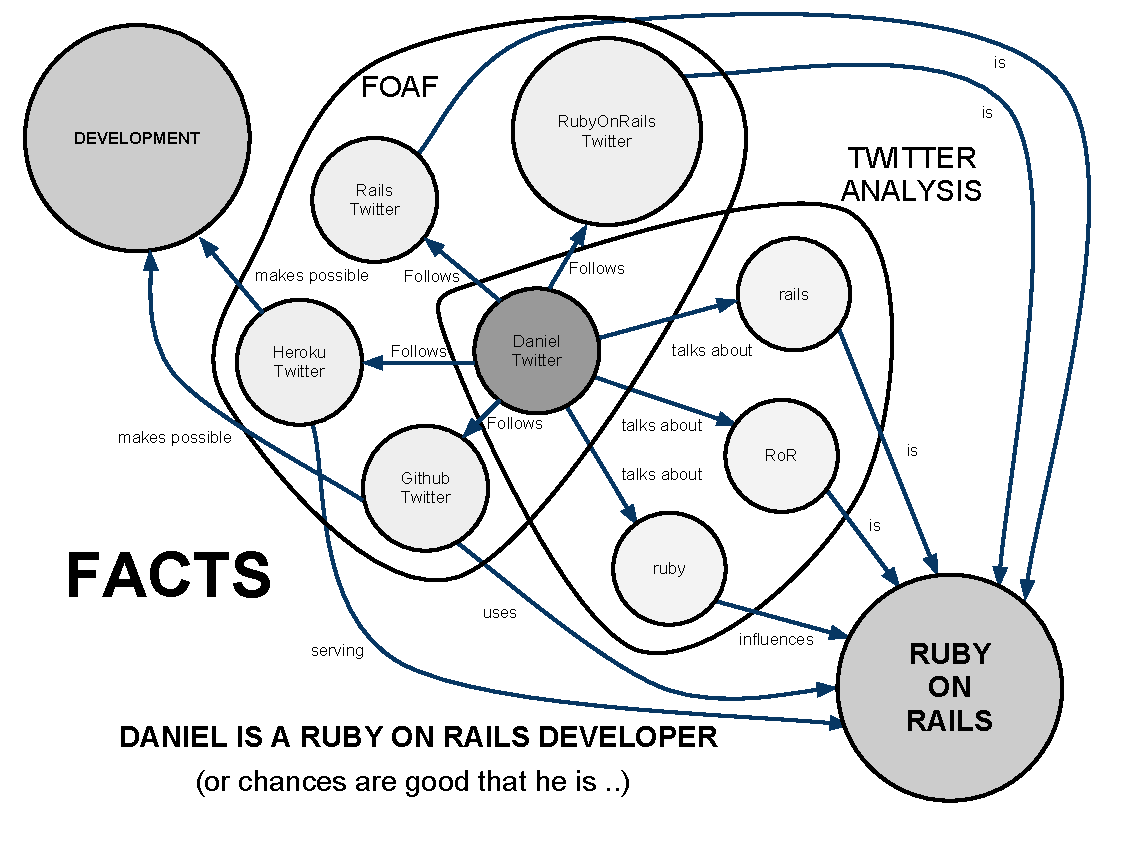
\includegraphics[width=1.0\textwidth]{./fig/makingsenseoftwitter.pdf}
	\caption{The internal representation of the entity Daniel, his relationships to other entities and the conclusions we can draw from analyzing these relationships: Daniel is a Ruby on Rails developer.}
	\label{fig:makingsenseoftwitter}
\end{figure}

By analyzing the available entities and their relationships, we would like to be able to conclude that Daniel is a Ruby on Rails developer. This is depicted in \autoref{fig:makingsenseoftwitter} by linking the subjects Daniel talks about to Ruby on Rails and the added knowledge that the entities Heroku and Github which Daniel follows, are both talking about development or to developers.

Using this information, we can create a mesh with links between entities. The number of useful links could then be part of the algorithm to determine the most influential Twitter users with regard to a specific topic.

\section{Expert Finding}
\label{expertfinding}


Finding experts is useful for seeking consultants, collaborators or speakers. It is also of great value within the academic world as it provides a source of information to supplement or complement papers and theses. Many researchers and reporters lose a lot of time doing this manually as the amount of sources is ever growing: documents, email, databases, conferences, scientific papers and so on. The topic is luckily seeing an increase in attention in recent years.

%Expert finding is a difficult task requiring a multitude of different steps in order to find results bearing certain value. There are databases containing records of people matched with their area of expertise, which can be queried for a nominal fee, mostly used by reporters. The data has been gathered manually over time. To receive a more up-to-date or specific result, one will have to send a separate request which will come with a higher price and take its time.\\
%Another option is to do it manually. There are several steps which can be undertaken and they can be executed in fashionable order, repeated as often as necessary. One can search for conference sites about the topic and look up the names of the speakers. Current and past working experience can possibly be found on LinkedIn. Publications and co-authors can be retrieved from online databases with dedicated research publications or from more general databases such as Google Scholar. The authors and papers can be interlinked in order to see who works with who and who is most often cited or referenced. Influence can be measured on social media.\\
%It is clearly a lengthy process.
\subsection{Current situation}

% Say something about using OWL, FOAF, RDF, triplestores ... Generally saying more about the 2 month we needed to actually get to our problem ...

Expert finding is a difficult task requiring a multitude of different steps in order to find results bearing certain value. There are databases containing records of people matched with their area of expertise, which can be queried for a nominal fee, mostly used by reporters. The data has been gathered manually over time. To receive a more up-to-date or specific result, one will have to send a separate request which will come with a higher price and take its time.

In research circles, \cite{balog2006finding} proposes four simple binary association methods to find expertise information from emails while \cite{liu2005finding} investigates the expertise of users and experts by combining information retrieval techniques. Both these solutions are insufficient for topic-based expert finding as their datasets (emails and online communities) are too limited, they focus too much on previous encounters and lack context.

\cite{mattox1999enterprise} retrieves experts based on the amount of documents persons have for a given topic. As input a keyword phrase is used in order to find relevant documents. The results are however unsatisfactory caused by its slow response time and incorrect relationship between persons and documents. \cite{zhu2006open} gets better results using an algorithm based on a PageRank for document authority, a co-occurrence model for authors and multiple levels of associations between experts and topics. It succeeds to map variants of experts' names on the same author, but fails to identify different authors with the same name.

\cite{jung2007finding} proposes OntoFrame. It is an information service platform using Semantic Web technologies and is based on an extensive ontology of 16 classes using RDF triples. Identity resolution and full text analysis forms the basis of their expert-finding method. The framework looks promising, however the prototype does not function  \cite{ontoframe}.

\subsection{Improvements and additions}

% TODO Iets vermelden over de connectie met het TWIRL project?

We want to continue the research proposed in \cite{balog2006finding}, but less focused towards the full text analysis of documents. We want to create a platform that extracts and unifies the required information from a variety of online sources and subsequently builds a repository of user profiles.

% TODO We looked into the usage of a triplestore in order to use OWL \autoref{owl} ... or sth like that ?

We will need to write a web scraper (see \autoref{scraping}) in order to retrieve information from online sources that do not provide a public API. This information will have to be stored and this storage should allow us to make and change connections between different entities and adding and combining them graciously. We choose to use the TinkerPop Graph, using the graph databases. For more information about graphs, see \autoref{graphs}.

In order to differentiate between authors with the same name and find similarities between publications that are written by the same author, we will use a clustering algorithm (as described in \autoref{clustering}). The nodes will be names we found in publications or on profiles and clusters will represent one author, mapping one or more names to the same author. This allows us to define rules which calculate the probability that names match the same author and using this new information in the clustering algorithm will lead to reformations in the graph space.

For the clustering algorithm, we focused on the algorithm proposed in \cite{saha2006dynamic}. This is an efficient, dynamic algorithm which can handle the flow of new information in the form of new nodes and new edges connecting these nodes. For the required minimum-cut tree algorithm, we based ourselves on the sequential Gusfield's algorithm explained in \cite{rodrigues2011mpi}. A very detailed elaboration of everything related to this clustering algorithm can be found in \autoref{clustering}.

We want to find experts about certain subjects. This means we have to find keywords related to publications. We will discuss different possibilities, but one is parsing the most important words from the title. We will do this by using a part-of-speech tagger, see \autoref{postagger}.

% TODO Te bespreken: neo4j, Tinkerpop, Gremlin, Stanford POS tagger, lemmatizer, doc split (ruby gem), resque (ruby library - https://github.com/defunkt/resque), max flow :: min-cut
